% !TEX root = ../../main.tex

\subsection{Vapour adsorption}

The effects of shaping with \(\rho\)-alumina are 
so far more subtle than the changes encountered when using 
PVA, as shown in the corresponding 
study~\cite{chanutObservingEffectsShaping2016}.
As such we extended the characterisation using adsorption
of vapours at room temperature.
The influence of the binder on hydrophobic character of the
material may be of interest for tuning the properties of the 
beads. Here, water and methanol
can serve as probes for small changes in surface properties.
To this end, the same PVA samples which were 
used in the previous study were investigated alongside 
the MRA-shaped MOF.

Due to its surface charges, alumina is a 
hydrophilic substance, with a contact 
angle of \SI{10}{\degree}. It is expected that its 
addition may therefore increase the affinity 
of the resulting pellet towards water. On the other hand,
the PVA binder is more hydrophobic, with a water contact
angle of \SI{51}{\degree}. The medium affinity for water
is due to the surface hydroxyl functionalizations, which
can lead to hydrogen bonding.

Two indicators may highlight changes in material hydrophilicity: 
the slope of the isotherm in the low relative pressure region 
(\(p/p^0 < 0.3\)) and condensation steps in the isotherm. 
Adsorption at low pressures is representative of the initial
interactions with the surface, as discussed in the previous section.
The pressure at which condensation occurs in the pores of the material, 
underlined by a sharp increase in the isotherm, depends on the 
size of the pore but also on pore environment and 
guest-guest interactions. Finally, hysteresis in the adsorption 
isotherm may also be an indication of the nature of pores.

The measured isotherms on water and methanol can be found
in \autoref{shaping:fgr:wateradsorption} 
and \autoref{shaping:fgr:methanoladsorption} respectively.
Initial Henry constants have been calculated for the isotherms
using the initial point method, and are displayed in
\autoref{shaping:fgr:vapourkh}.

\begin{figure}[htb]
    \centering
    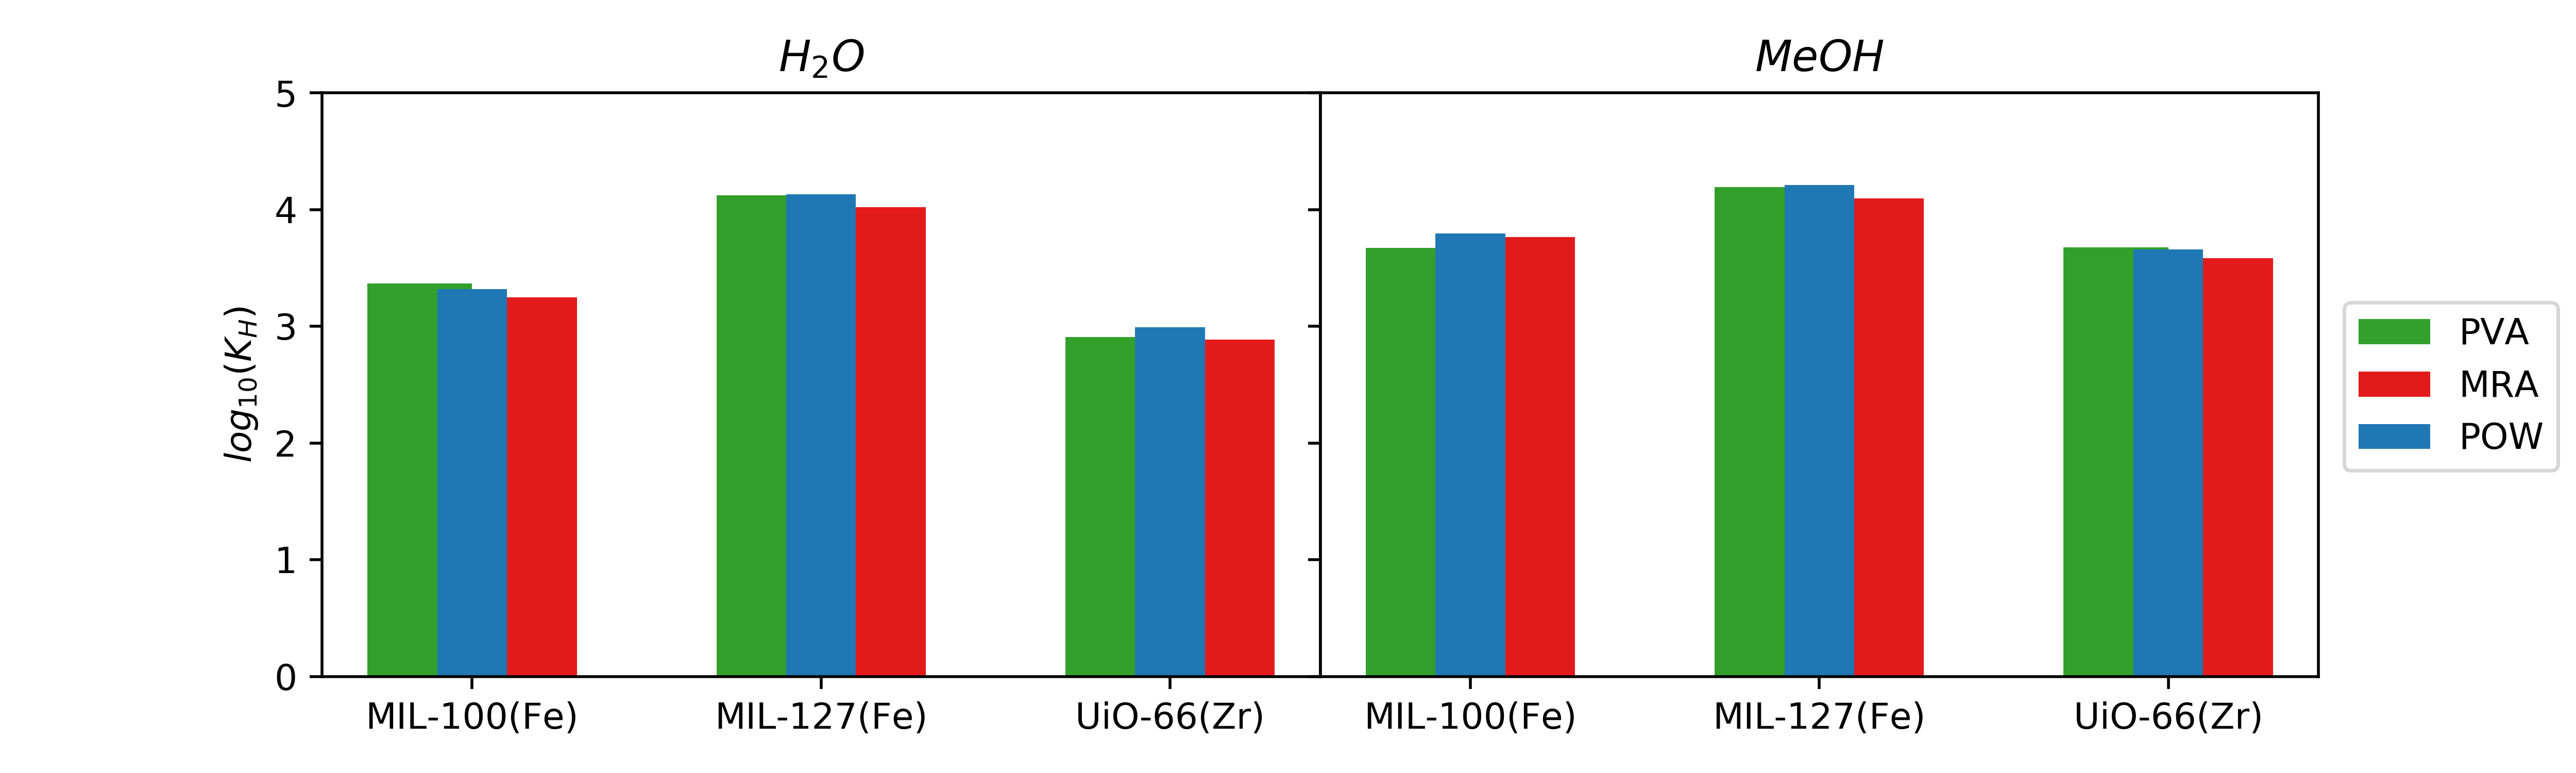
\includegraphics[width=\linewidth]{vapourkh}%
    \caption{Calculated initial Henry constant for
    the vapour adsorption isotherms 
    in \autoref{shaping:fgr:wateradsorption}
    and \autoref{shaping:fgr:methanoladsorption}}%
    \label{shaping:fgr:vapourkh}
\end{figure}

\subsubsection{UiO-66(Zr)}

On the parent UiO-66(Zr), the water isotherm shows a slow uptake 
at the start, indicating a hydrophobic surface, and then shows 
a small step at \(p/p^0 = 0.3\). While little is 
adsorbed on the MOF before this step, its presence 
at a low relative humidity is indicative of intrinsic defects
in the framework~\cite{ghoshWaterAdsorptionUiO662014}.
Complete saturation takes place around \(p/p^0 = 0.9\). 
A wide hysteresis curve can be seen, which 
does not fully close, even at low pressures. Both the
saturation step and the condensation may be attributed 
to agglomeration of crystals and interparticle voids.

The methanol isotherm has the same features as the water
one, with the condensation step shifted at a much lower 
partial pressure (\(10^{-1} p/p^0\)). It is likely that
the organic component of methanol interacts with the
hydrophobic surface, thus permitting pore filling at
lower pressures. This is also evidenced through the higher
Henry constant when compared to water.

When comparing the powder and the pellet variants, the 
general shape of the isotherm remains the same with both
water and methanol. Initial interactions with the surface are also
identical, as evidenced by the overlap in the low pressure region
and through the calculated Henry constants. The isotherms 
begin to diverge after the condensation step, where the 
maximum loading evolves in the order MRA < powder < PVA
for both vapours. This is a surprising trend, as both pellets
have been shown to have lower capacities than the powder,
stemming from material amorphization during granulation.
The addition of hydrophilic alumina conforms to this hypothesis,
and appears to have no impact on the initial interaction with 
the surface. On the other hand, polymer-shaped particles
seem to have a higher maximum capacity than both powder and 
alumina pellets. It is unclear if this effect is due to a 
cooperative effect of hydrogen bonding with hydroxyl groups 
on the polymer chains or has another underlying cause.

\todo{technically it is not an apples to apples comparison
as the alumina and pva pellets had different starting materials...}


\begin{figure}[p!]
    \centering

    \begin{subfigure}{\linewidth}
        \centering
        \parbox{0.1\linewidth}{\caption{}\label{shaping:fgr:wateruio66}}%
        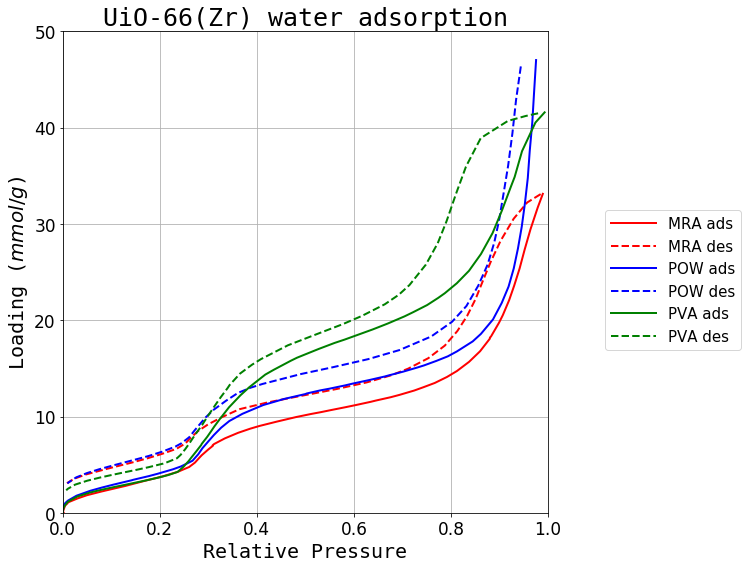
\includegraphics[width=0.4\textwidth]{water/UiO-66(Zr)-water}%
        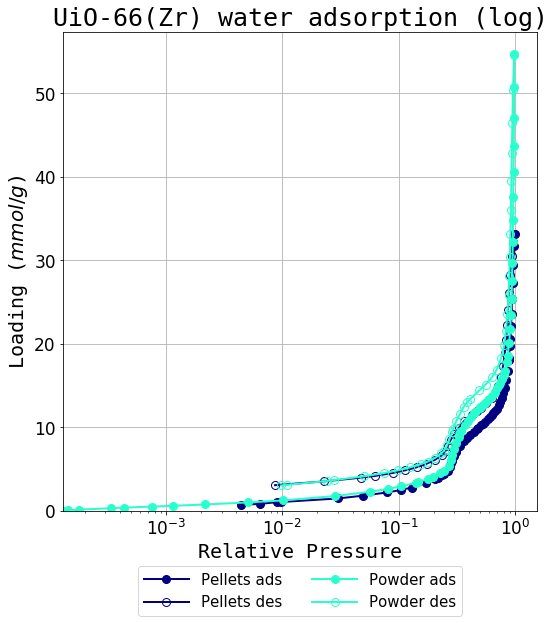
\includegraphics[width=0.4\textwidth]{water/UiO-66(Zr)-water-log}%
    \end{subfigure}%

    \begin{subfigure}{\linewidth}
        \centering
        \parbox{0.1\linewidth}{\caption{}\label{shaping:fgr:watermil100}}%
        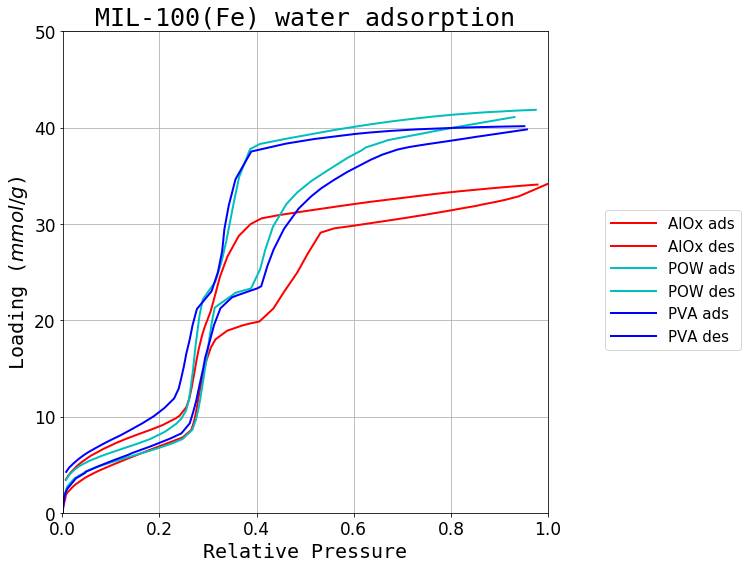
\includegraphics[width=0.4\textwidth]{water/MIL-100(Fe)-water}%
        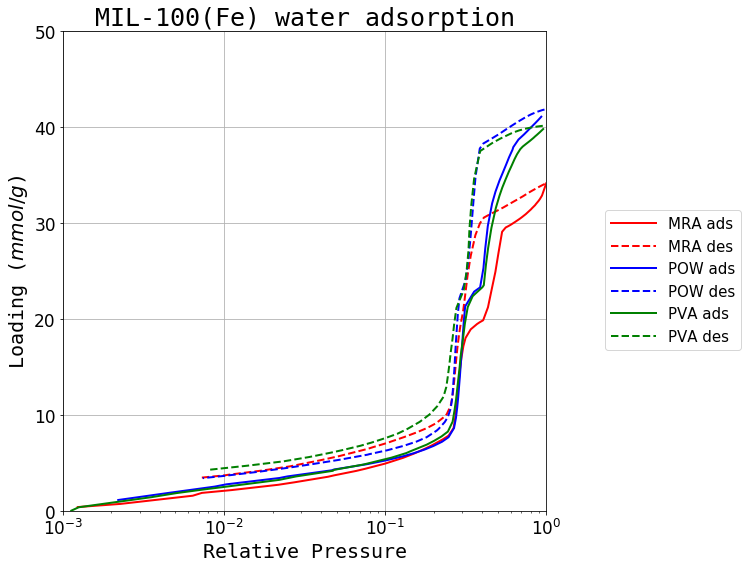
\includegraphics[width=0.4\textwidth]{water/MIL-100(Fe)-water-log}%
    \end{subfigure}%

    \begin{subfigure}{\linewidth}
        \centering
        \parbox{0.1\linewidth}{\caption{}\label{shaping:fgr:watermil127}}%
        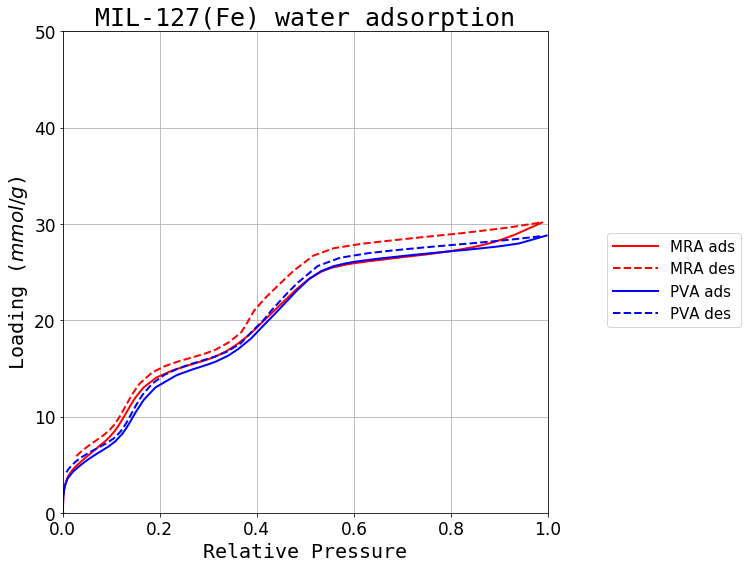
\includegraphics[width=0.4\textwidth]{water/MIL-127(Fe)-water}%
        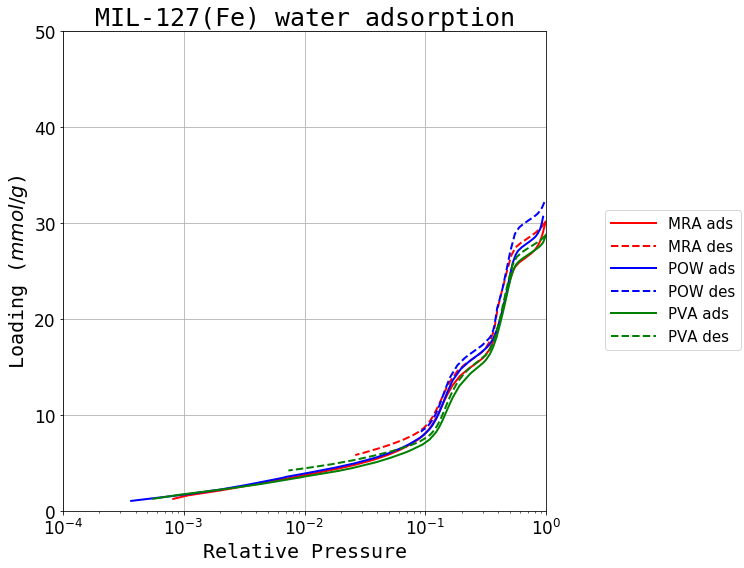
\includegraphics[width=0.4\textwidth]{water/MIL-127(Fe)-water-log}%
    \end{subfigure}%
    
    \caption{Water adsorption isotherms (a) UiO-66(Zr), 
    (b) MIL-100(Fe) and (c) MIL-127(Fe). The powder samples are in light
    blue, while the \(\rho\)-alumina and poly-vinyl alcohol samples are in red
    and dark blue respectively. Logarithmic graphs of the isotherms are
    on the right for clarity of the low
    pressure region.}%
    \label{shaping:fgr:wateradsorption}
\end{figure}

\subsubsection{MIL-100(Fe)}

The water isotherm on the powder MIL-100(Fe) material show a more 
hydrophilic environment, with a higher initial uptake, and two 
condensation steps at \(p/p^0 = 0.3\) and \(p/p^0 = 0.5\).
At low pressures, adsorption takes place on metal sites in the 
large cages, with clusters formed around these hydrophilic
sites. The two steps correspond to the successive filling of the 
\SI{25}{\angstrom} and the \SI{29}{\angstrom} pores. The
adsorption and desorption branches show a hysteresis loop 
formation, associated with the condensation in the largest 
mesoporous spherical pore.

The methanol isotherm on the same parent MOF still presents 
two condensation steps, which have been shifted at to 
lower pressure. There is no longer any hysteresis present,
an indication that the critical pore radius for its formation
is not attained when using methanol.

If comparing the powder isotherms with their shaped counterparts,
no differences in features are visible. Initial Henry's constant 
is similar with all  

\subsubsection{MIL-127(Fe)}

On the last MOF powder, the water isotherm shows a hydrophilic
surface, with a highest initial slope out of the three 
materials studied. The isotherm has two condensation steps,
a low relative humidity one at \(0.15~p/p^0\), which corresponds
to the filling of the hydrophilic pore, and a condensation 
step situated at \(0.5~p/p^0\) inside the hydrophobic micropore.
No hysteresis is observed.

As a striking difference from water behaviour, methanol adsorption
leads to completely filled pores at below \(0.15\) relative 
pressure. By examining the logarithmic isotherms in 
\autoref{shaping:fgr:methanolmil127} a steep slope at low
pressures is evident. It is likely that the larger size of the
methanol molecule is much more affected by confinement in 
the hydrophilic pore, and leads to sudden micropore filling.
The same effect, combined with the increased affinity for the 
organic part of the probe is likely responsible for shifting the 
secondary condensation step at lower pressures.

The similarities between the both variants of shaped pellets 
and the original powder confirms the previously observed 
suitability of this MOF towards the shaping process. The isotherms
overlap almost fully, with a slight difference in maximum uptake
in the order of powder > PVA > alumina.

\begin{figure}[p!]
    \centering

    \begin{subfigure}{\linewidth}
        \centering
        \parbox{0.1\linewidth}{\caption{}\label{shaping:fgr:methanoluio66}}%
        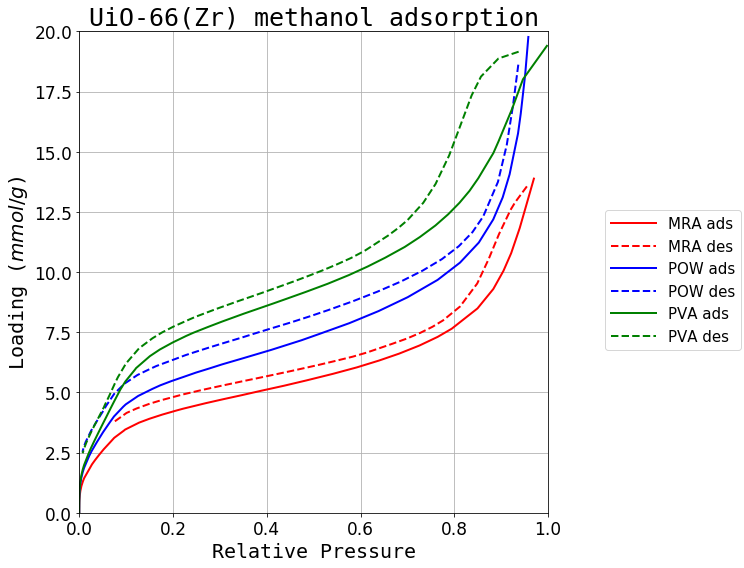
\includegraphics[width=0.4\textwidth]{methanol/UiO-66(Zr)-methanol}%
        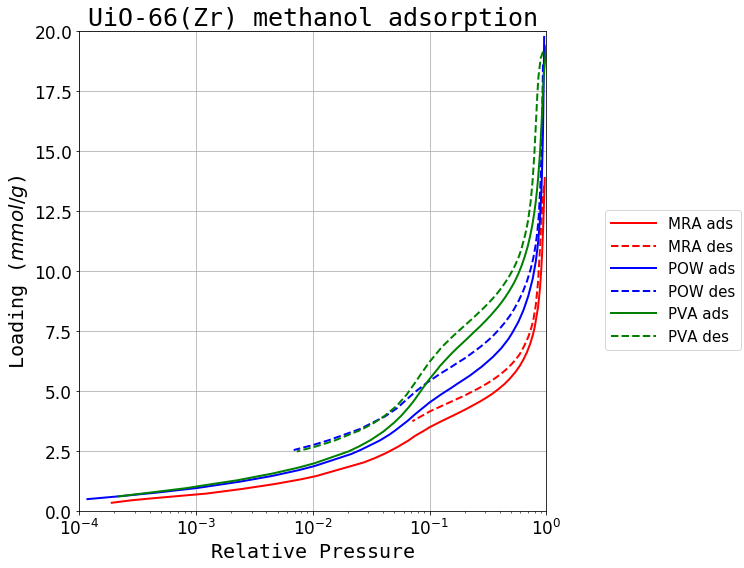
\includegraphics[width=0.4\textwidth]{methanol/UiO-66(Zr)-methanol-log}%
    \end{subfigure}%

    \begin{subfigure}{\linewidth}
        \centering
        \parbox{0.1\linewidth}{\caption{}\label{shaping:fgr:methanolmil100}}%
        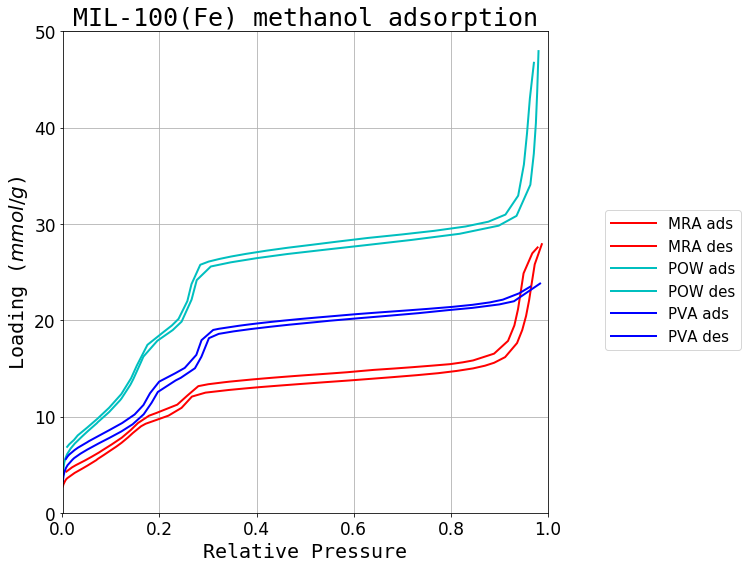
\includegraphics[width=0.4\textwidth]{methanol/MIL-100(Fe)-methanol}%
        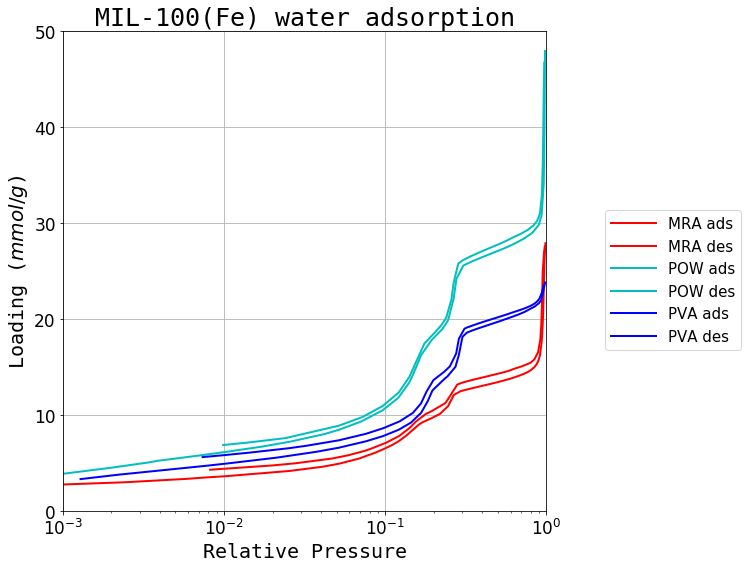
\includegraphics[width=0.4\textwidth]{methanol/MIL-100(Fe)-methanol-log}%
    \end{subfigure}%

    \begin{subfigure}{\linewidth}
        \centering
        \parbox{0.1\linewidth}{\caption{}\label{shaping:fgr:methanolmil127}}%
        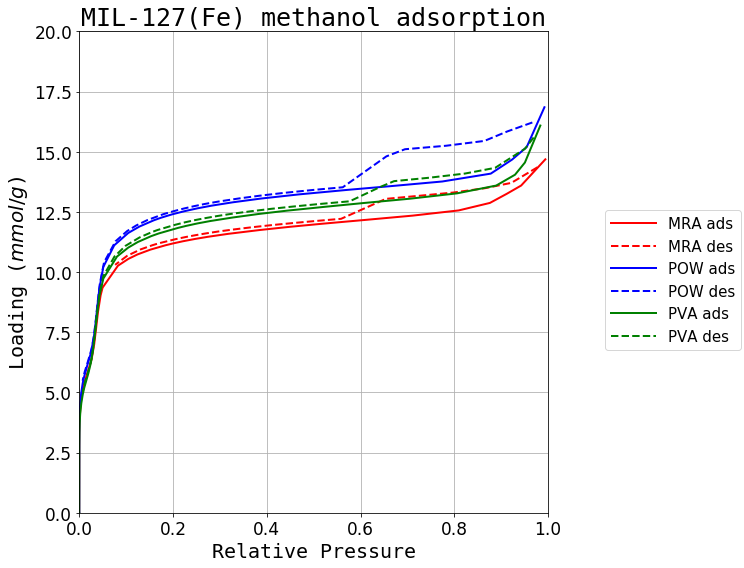
\includegraphics[width=0.4\textwidth]{methanol/MIL-127(Fe)-methanol}%
        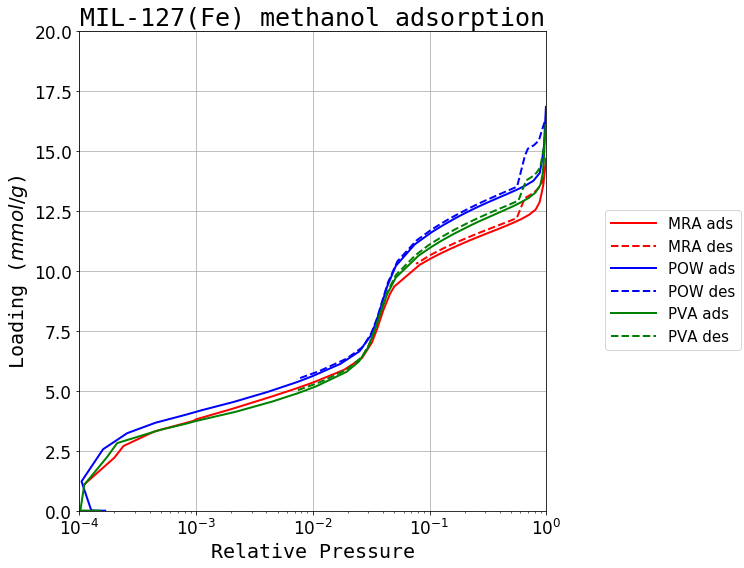
\includegraphics[width=0.4\textwidth]{methanol/MIL-127(Fe)-methanol-log}%
    \end{subfigure}%
    
    \caption{Methanol adsorption isotherms (a) UiO-66(Zr), 
    (b) MIL-100(Fe) and (c) MIL-127(Fe). The powder samples are in light
    blue, while the \(\rho\)-alumina (MRA) and poly-vinyl alcohol 
    (PVA) samples are in red and dark blue respectively. Logarithmic 
    graphs of the isotherms are on the right for clarity of the low
    pressure region.}%
    \label{shaping:fgr:methanoladsorption}
\end{figure}